\documentclass[8pt]{article}

\usepackage[T1]{fontenc}
\usepackage[utf8]{inputenc}
\usepackage{graphicx}
\usepackage{lmodern}
\usepackage{amsmath}
\usepackage{xfrac}
\usepackage{amsthm}
\usepackage{listings}
\usepackage{enumerate}
\usepackage{amssymb}
\usepackage{cancel}
\usepackage{amsfonts}
\usepackage{float}
\usepackage{fullpage}
\usepackage{pdfpages}
\usepackage{tcolorbox}

\DeclareUnicodeCharacter{200A}{ } 
\renewcommand*\contentsname{Table des matières}

\PassOptionsToPackage{hyphens}{url}\usepackage{hyperref}

\usepackage{listings}
\author{ControverSciences\textit{ et al} }
\title{Projet AREN - Corpus de ressources \\   Opérations militaires extérieures de la France.}
\date{24 Mars 2019}

\begin{document}
\maketitle

Ce corpus de ressources et de textes à débattre étudiera les outils techniques dont dispose l’armée française lors d'opérations militaires extérieures, en particulier à travers l'exemple des drones. Les sujet est abordé par la définition des opérations militaires extérieures de la France, ainsi que le cadre légal et financier dans lequel il s'exerce (\ref{sec:definition}). Ensuite, un article de \textit{CNRS Le Journal} aborde la définition et les enjeux des armes létales autonomes (\ref{sec:autonome}). Enfin un article complet et long de la revue \textit{Pour La Science} permet à celles et ceux qui souhaitent d'approfondir les enjeux et l'utilisation des drone et armes létales autonomes dans les conflits extérieurs (\ref{sec:machines}).\\


Ce corpus de préparation permet d'aborder les différentes facettes du débat sur l'utilisation des drones dans les opérations militaires extérieures de la France. Deux textes sont proposés pour le débat, et peuvent être coupés afin d'extraire les paragraphes suffisants au débat. Le premier est en article du journal \textit{Le Parisien} sur l'utilisation des drone dans la lutte contre le terrorisme, avec l'exemple de la mort de Fabien Clain (\ref{sec:Fabien_Clain}). Le second est un article du journal \textit{Le Monde} sur l'utilisation de drone munis de bombe, qui seront utilisés au Sahel à la fin de l’année 2019 par l'armée française (\ref{sec:france_drone}). 

\tableofcontents
\newpage
\section{Corpus de ressources}
\subsection{Les opérations militaires extérieures de la France (OPEX)}
\label{sec:definition}

\begin{itemize}
	\item \textbf{Lien~: }  \url{https://www.vie-publique.fr/actualite/dossier/defense/operations-militaires-exterieures-france-opex.html} 
	\item \textbf{Auteur~: } Vie-publique.fr
	\item \textbf{Date~: } 14 août 2018 
	\item \textbf{Source~: } Vie-publique.fr est produit, édité et géré par la direction de l'information légale et administrative (sous l'autorité du Premier ministre et rattachée au secrétaire général du gouvernement). Ce portail pour but de faciliter l’accès des citoyens aux ressources et données utiles pour appréhender les grands sujets qui animent le débat public français. 
	\item \textbf{Résumé~: }Irak, Syrie, Centrafrique, Sahel, les opérations militaires extérieures sont devenues une composante structurelle de l’activité opérationnelle des armées, en particulier de l’armée de terre.
	
	Comment sont-elles préparées ? Quels sont leurs cadres d’intervention ? Comment sont-elles financées et quelle est la condition des militaires en opérations extérieures (OPEX) ?
\end{itemize}

\textbf{Que sont les OPEX ?} \\

D’après la définition traditionnelle donnée par le Ministère des armées, les opérations extérieures sont les “interventions des forces militaires françaises en dehors du territoire national”.\\

La qualification d’OPEX résulte d’un arrêté du ministre des armées, qui porte ouverture du théâtre d’engagement en précisant la zone géographique et la période concernées. Les OPEX se distinguent des forces prépositionnées dans des bases en Afrique en vertu d’accords de défense ou en mer.\\

En amont du déploiement des forces, le Centre de planification et de conduite des opérations fait diverses propositions de noms d’opérations, parmi lesquelles la présidence de la République choisit la dénomination retenue in fine. Les opérations récentes ont pour nom Harmattan (Libye, 2011), Serval (Mali, 2013), Sangaris (République centrafricaine, 2013), Barkhane (Sahel, 2014) ou Chammal (Irak, Syrie, 2014).\\

Depuis 1995, les armées françaises ont été engagées dans quelque 106 opérations menées à l’extérieur des frontières nationales. A ces opérations, il convient d’ajouter 5 opérations lancées antérieurement à cette date mais toujours en cours~: en Israël (depuis mai 1948), au Liban (1978), au Sinaï (1982), dans le golfe de Guinée (1990) et au Sahara occidental (1991).\\

Les OPEX se déroulent dans le cadre~:

\begin{itemize}
	\setlength\itemsep{-0.25em}
	\item de l’ONU~: Liban (opération Daman menée dans le cadre de la Finul), Côte d’Ivoire (Onuci), Sahara occidental (Minurso), Liberia (Minufil), République démocratique du Congo (Monusco)~;
	\item de l’Union européenne~: mandat de la Mission de sécurité européenne pour l’assistance à réforme de la sécurité en République démocratique du Congo (EUSEC) achevé en juin 2016~; opération Atalanta (2008) de lutte contre la piraterie maritime au large de la Corne de l’Afrique~;
	\item de forces multinationales, comme la Force multinationale d’observation (FMO) dans le Sinaï~;
	\item de forces multinationales, comme la Force multinationale d’observation (FMO) dans le Sinaï~;
	et dans un cadre national (équipes de protection embarquées sur des bateaux thoniers-seniers de sociétés d’armateurs privés français).
\end{itemize}


\textbf{Qui décide et contrôle les OPEX ?}\\

La décision d’engagement des armées est prise par le Président de la République en Conseil de défense sur le fondement des prérogatives qu’il tient de l’article 15 de la Constitution du 4 octobre 1958 et de l’article 5, alinéa 2, qui fait de lui le “garant de l’indépendance nationale, de l’intégrité du territoire et du respect des traités”.\\

Les ordres d’opération et la directive administrative et logistique sont produits par l’état-major des armées. La directive précise le périmètre géographique du théâtre d’opérations et ses modalités de soutien, dont le soutien financier (affectation des dépenses aux budgets opérationnels de programmes OPEX et versement de l’indemnité de sujétion pour service à l’étranger, notamment).\\

\textbf{Le contrôle parlementaire des OPEX}\\

Avec la modification des dispositions de l’article 35 de la Constitution, la réforme constitutionnelle du 23 juillet 2008 a renforcé le contrôle parlementaire.\\

Si le gouvernement décide d’engager une intervention armée, il doit informer le Parlement dans les trois jours. Un débat parlementaire sans vote peut être organisé, comme ce fut le cas le 24 septembre 2014 lors de l’intervention de la France en Irak avec l’opération Chammal ou le 25 septembre 2015 lors de l’engagement des forces aériennes en Syrie. Si l’intervention extérieure se prolonge au-delà de quatre mois, le gouvernement soumet cette prolongation à l’autorisation du Parlement. Il peut demander à l’Assemblée nationale de décider en dernier ressort.\\

\begin{center}
	\makebox[\textwidth]{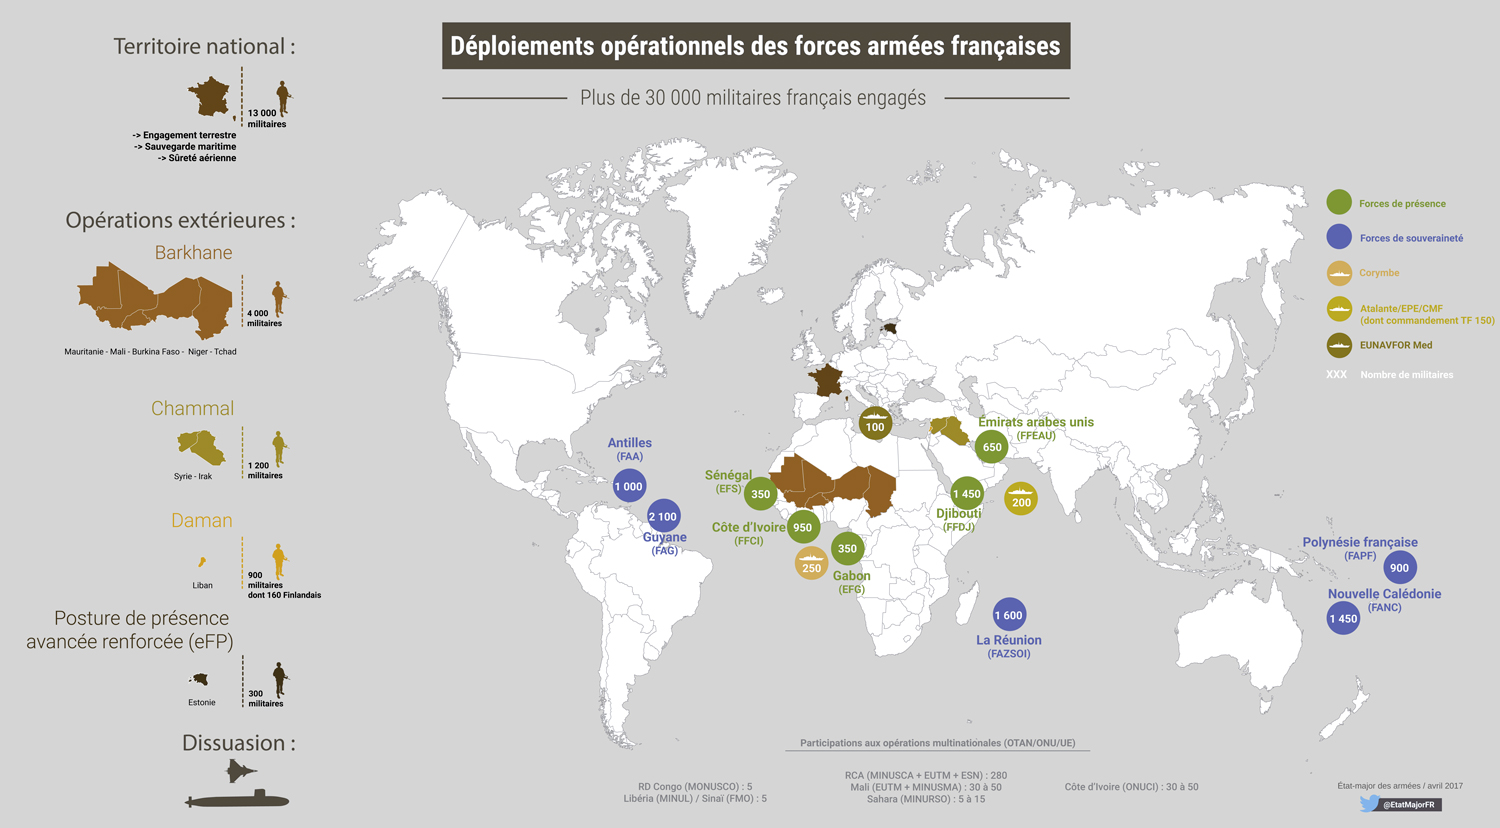
\includegraphics[width=1.0\textwidth]{deploiementdesarmees}}
\end{center}

Depuis l’entrée en vigueur de cette disposition, le gouvernement a demandé à sept reprises la prolongation d’une intervention extérieure~:
\begin{itemize}
	\setlength\itemsep{-0.25em}
	\item le 22 septembre 2008 demande de prolongation de l’intervention en Afghanistan~;
	\item le 28 janvier 2009 demande de prolongation de cinq interventions (Côte d’Ivoire, Tchad, \item Liban, Kosovo, République Centrafricaine)~;
	\item le 12 juillet 2011 demande de prolongation de l’intervention en Libye~;
	\item le 22 avril 2013, demande de prolongation de l’opération Serval au Mali~;
	\item le 25 février 2014 demande de prolongation de l’opération Sangaris en République Centrafricaine~;
	\item le 13 janvier 2015, demande de prolongation de l’opération Chammal en Irak~;
	\item le 25 novembre 2015, demande de prolongation de l’engagement des forces aériennes au-dessus du territoire syrien.
\end{itemize}



\textbf{La budgétisation et le financement des OPEX}\\

Dans son rapport de novembre 2016 sur les OPEX, la Cour des comptes constate une modification de la nature et du coût des OPEX entre 2012 et 2015. Ces engagements armés se déploient selon des formats, intensités et durées variables, avec des répercussions quant à l’affectation des dépenses~: sur quels budgets affecter les dépenses d’entraînement de l’armée afghane ou la protection des navires au large de la Somalie ?\\

La Cour des comptes souligne que les dépenses supplémentaires dues aux OPEX ont représenté, au cours des trois derniers exercices, plus de 1,1 milliard d’euros chaque année. Le coût unitaire, par militaire projeté, d’une opération extérieure a plus que doublé depuis une décennie, pour atteindre plus de 100 000 d’euros par soldat déployé par an.\\

La Cour des comptes comme le Sénat (rapport d’octobre 2016) demandent une meilleure connaissance du surcoût croissant des OPEX et recommandent d’inscrire en loi de finances initiale une dotation réaliste et sincère pour les OPEX.\\

La loi de programmation militaire 2019-2025 du 13 juillet 2018 consacre la remontée de l’effort de défense de la France, voulue par le président de la République, pour faire face aux menaces décrites par la Revue stratégique d’octobre 2017.\\

Outre l’augmentation prévue au budget général, la loi de programmation militaire (LPM) prévoit que le ministère des Armées prenne progressivement en charge l’intégralité du coût des opérations extérieures, jusqu’ici partiellement financé par d’autres ministères.
La protection sociale des militaires en OPEX et le devoir de mémoire.\\

\textbf{Le régime de rémunération des militaires en OPEX}\\

Selon le rapport de la Cour des comptes de novembre 2016, l’indemnité pour sujétion de services à l’étranger (ISSE) s’élevait à 291,3 millions en 2015 et concernait un effectif de 8 160 personnes. Le montant moyen annuel de l’ISSE s’élève 35 000 euros par militaire.\\

Les OPEX durent en général quatre mois. Depuis le 1er octobre 2015, la carte de combattant est attribuée à tous les militaires ayant servi pendant au moins quatre mois (120 jours cumulatifs de présence) en opération extérieure.\\

Le rapport de la Cour des comptes précise que “la rémunération brute globale en OPEX est, selon le grade et la situation de famille, de 1,9 à 2,3 fois plus élevée que celle qu’il perçoit habituellement”. L’ISSE n’est par ailleurs pas prise en compte pour le calcul de l’impôt sur le revenu, mais elle est assujettie à la CSG, au RDS et à la cotisation de solidarité.\\

\textbf{Un accompagnement social spécifique des militaires et de leur famille}\\

Dans son 11e rapport (décembre 2017), le Haut Comité d’évaluation de la condition militaire recense 154 militaires morts en opérations extérieures de 2007 à 2016. Selon le Service de santé des armées, le nombre de militaires blessés lors des opérations extérieures s’élève à 620 de 2007 à 2016.\\

Pour la prise en compte des blessures psychiques (syndrome de stress post-traumatique - SSPT), les OPEX comportent, depuis 2010, un volet dédié au soutien psychologique, avec un référent psychologique au niveau de chaque section, un officier “environnement humain” pour le bataillon et un psychologue à l’échelle du théâtre d’opérations.\\

\textbf{Un monument en hommage aux soldats morts en opérations extérieures}\\

Le 18 avril 2017, le président de la République François Hollande a posé la première pierre du monument en l’honneur des militaires tombés en opérations extérieures de 1963 à ce jour. Les noms de ces soldats morts pour la France (dont la liste n’a pas encore été finalisée) doivent figurer en lettres d’or sur un mur de marbre noir situé dans le parc André-Citroën (XVe arrondissement de Paris). Dans son discours aux armées le 13 juillet 2018, Emmanuel Macron a annoncé avoir relancé le projet de ce monument.




\newpage

\subsection{Armes létales autonomes: de quoi parle-t-on?}
\label{sec:autonome}

\begin{itemize}
	\setlength\itemsep{-0.25em}
	\item \textbf{Lien~: }  \url{https://lejournal.cnrs.fr/billets/armes-letales-autonomes-de-quoi-parle-t} 
	\item \textbf{Auteur~: } Raja (Roboticien) Chatila et Catherine Tessier (chercheuse en intelligence artificielle). 
	\item \textbf{Date~: }  19 Octobre 2017
	\item \textbf{Source~: } CNRS Le journal, l'objectif de ce site est de partager largement avec les amateurs de science, les professeurs et leurs élèves, les étudiants et tous les citoyens curieux, des contenus destinés jusque-là à la communauté des agents du CNRS, chercheurs, ingénieurs et techniciens, ceux des labos comme ceux des bureaux.
	\item \textbf{Résumé~: }
	Le débat entourant le développement d’armes autonomes est biaisé par le caractère anxiogène des arguments. Mais pour pouvoir adopter une position sur le sujet, il faut en comprendre les enjeux précis. C’est ce que nous proposent les chercheurs Raja Chatila et Catherine Tessier. 
\end{itemize}

Les «~armes autonomes~», quand ce ne sont pas les «~robots-tueurs~», font l’objet, depuis environ trois ans, de nombreux articles de presse, lettres ouvertes et débats, dont on constate le caractère sensationnel et anxiogène des arguments avancés, ainsi que la quasi-absence d’explications et d’arguments scientifiques et techniques. Depuis 2014, le débat est engagé à l’ONU à Genève, dans le cadre de la Convention sur certaines armes classiques (CCAC), sur la question d’une interdiction ou d’un moratoire sur le développement de telles armes.\\

\textbf{Des mots à la réalité}\\

Le vocable de «~robot-tueur~» suggère que le robot serait animé par l’intention de tuer, voire qu’il en serait conscient, ce qui n’a évidemment pas de sens pour une machine, quand bien même elle a été conçue et programmée pour détruire, neutraliser ou tuer~: on ne parle pas, par exemple, de «~missile-tueur~». Il s’agit là d’une rhétorique du pathos qui entrave par nature la discussion éthique, mais qui est utilisée pour rechercher un effet de rejet du public.\\

Le terme «~autonome~» est également problématique parce que les différentes parties prenantes, et en premier lieu les scientifiques, lui accordent des acceptions multiples. Une «~arme autonome~» peut ainsi désigner un engin qui réagit automatiquement à certains signaux prédéfinis, ou bien qui optimise sa trajectoire pour atteindre un objectif dont il aura reconnu automatiquement une signature prédéfinie, ou encore qui cherche automatiquement dans une zone donnée une cible spécifiée par certaines caractéristiques.\\

Plutôt donc que de parler d’ «~arme autonome~», il semble plus pertinent d’étudier quelles fonctions sont – ou pourront être – automatisées, c’est-à-dire assignées à des programmes informatiques, et avec quelles limitations, dans le cadre d’un partage de l’autorité avec un opérateur humain.\\

\textbf{Les fonctions automatisées}\\

Les fonctions de guidage et de navigation sont depuis longtemps automatisées (pilotage automatique des avions ou des drones, par exemple) et n’ont pas soulevé de questionnement notable~; elles sont non critiques pour ce débat. Plus sensibles sont les fonctions d’identification et d’engagement (c’est-à-dire d’ouverture du feu) automatiques de cibles.\\

Les armes existantes, qui sont dotées de capacités de reconnaissance de cibles, sont équipées de logiciels qui comparent des signaux perçus par les capteurs (radio, radars, caméras, etc.) avec une base de signatures (modèles prédéfinis de cibles). Cela concerne en général de gros objets «~faciles~» à reconnaître (radars, bases aériennes, chars, batteries de missiles). L’engagement des cibles est réalisé sous supervision humaine. En revanche, ce type de logiciels ne permet pas d’évaluer la situation aux alentours de ces objets – par exemple, la présence de civils.\\

\textbf{Reconnaître des cibles complexes}\\

Les discussions et controverses actuelles portent sur le fait qu’une arme puisse être dotée de la capacité de reconnaître des cibles plus complexes (par exemple, des combattants par rapport à des blessés hors de combat), dans des situations et des environnements eux-mêmes complexes (par exemple, dans une situation évolutive), et de la capacité d’engager de telles cibles sur la seule base de cette reconnaissance.\\

De telles capacités supposeraient de disposer d’une description formelle (mathématique) des états possibles de l’environnement, des éléments d’intérêt et des actions à effectuer, sachant qu’il n’y a pas de situation type. Elles supposeraient également de reconnaître, à partir des capteurs, tel état, tel élément d’intérêt, et d’évaluer si les actions envisagées respectent les principes d’humanité (éviter les maux superflus), de discrimination (distinguer les objectifs militaires des populations et biens civils), et de proportionnalité (adéquation entre les moyens mis en œuvre et l’effet recherché) inscrits dans le droit international humanitaire (DIH). Les difficultés sont liées au fait de pouvoir comprendre automatiquement une situation sur la base de modèles mathématiques.\\

\textbf{À qui revient la décision ?}\\

Au-delà des aspects techniques et légaux, est-il éthiquement admissible que la décision de supprimer un être humain identifié par une machine soit confiée à cette machine ? Plus précisément, on doit se demander comment et par qui seraient établies la caractérisation, la modélisation et l’identification des objets d’intérêt, ainsi que la sélection de sous-ensembles d’informations (au détriment de certaines autres) pour calculer automatiquement la décision. Il s’agit également de savoir qui spécifierait ces algorithmes et comment il serait démontré qu’ils sont conformes aux conventions internationales et aux règles d’engagement, surtout s’ils sont capables d’apprentissage. En outre, qui devrait être responsable en cas de violation des conventions ou de détournement d’usage ? Car, au-delà des armes proprement dites, il est également important de réfléchir, lors de leur conception, aux potentiels détournements d’usage d’objets dits «~autonomes~» à des fins d’attaque. Par exemple, comment la voiture autonome ou le drone de loisir peuvent-ils être rendus robustes au piratage et à la modification malveillante ?\\

\textbf{Définir un cadre}\\

Face à ces questions, plusieurs organisations internationales appellent à ce qu’une arme dite «~autonome~» soit toujours sous contrôle humain significatif, c’est-à-dire que la décision d’engager une cible soit toujours prise par un être humain. D’un point de vue technique, il faut vérifier qu’un être humain dispose, en toutes circonstances, des informations suffisantes et du temps pour prendre cette décision, et cerner en quoi les informations calculées, sélectionnées et transmises par la machine influencent l’appréciation et la décision humaines.Ainsi, les préconisations formulées par la «~IEEE Global Initiative on Ethics of Autonomous and Intelligent Systems~», qui portent sur l’ensemble des technologies des systèmes autonomes et intelligents, énoncent pour les systèmes d’armes létales autonomes quelques principes dont la prévisibilité, la traçabilité, ou l’identification claire des responsabilités humaines. \\

Les systèmes adaptatifs et apprenants devraient ainsi être conçus de sorte qu’ils puissent expliquer leur raisonnement et leurs décisions aux opérateurs humains de manière compréhensible, les opérateurs demeurant responsables de la mise en œuvre de ces dispositifs. De plus, des systèmes autonomes au comportement prévisible pourraient devenir imprévisibles dans un déploiement en essaim où un comportement émergent imprévu peut apparaître. Ce type d’usage devrait donc être proscrit.\\

Enfin, il faut souligner que si les armes autonomes peuvent aider à gagner une guerre, l’effet psychologique de leur usage sur les populations qui en seront victimes risque fort d’empêcher de gagner la paix.\\

\newpage
\subsection{La guerre des machines}
\label{sec:machines}

\begin{itemize}
	\item \textbf{Lien~: }  \url{https://www.pourlascience.fr/sd/robotique/la-guerre-des-machines-2641.php} 
	\item \textbf{Auteur~: } Peter Singer, spécialiste
	de questions militaires.
	Il dirige le groupe de réflexion
	21st Century Defense Initiative
	(Initiative pour la défense
	au XXIe siècle) à la Brookings
	Institution, un centre
	de recherche en sciences
	sociales et politiques basé
	à Washington, aux États-Unis.
	\item \textbf{Date~: }  Juin 2011 
	\item \textbf{Source~: } Pour La Science est la version française du mensuel Scientific American. C'est une revue de vulgarisation scientifique dans toutes les disciplines, dont les articles sont signés par les chercheurs eux-mêmes.
	\item \textbf{Résumé~: } L'arrivée des robots sur les champs de bataille bouleverse la pratique de la guerre. Comme l'avènement des armes nucléaires, elle suscite aussi des questions d'ordre politique, juridique ou éthique.
\end{itemize}

L’histoire du robot militaire est liée à celle de l’auvsi. L’Association internationale pour les systèmes de véhicules sans pilotes (en anglais Association for Unmanned Vehicle Systems International ou auvsi) naît au début des années 1970 après l’utilisation des premiers drones de reconnaissance durant la guerre du Viêtnam. Quelques ingénieurs, chercheurs et officiers américains la fondent alors pour convaincre le Pentagone et le public de l’intérêt d’employer sur un champ de bataille des machines autonomes.\\

Au début, l’auvsi n’était qu’un obscur cercle de réflexion, qui se réunissait une ou deux fois par an pour discuter de questions techniques, créer des liens et échanger des on-dit. Toutefois, cette association a connu au cours des années 2000 une expansion fulgurante. Elle compte aujourd’hui 6 000 membres travaillant dans 1 500 entreprises et organismes répartis dans 55 pays.\\

Cette croissance est à mettre en parallèle avec l’un des changements les plus profonds dans les pratiques de la guerre depuis l’invention de la poudre ou des avions~: l’essor de l’utilisation de robots, par les plus puissantes armées du monde, a été étonnamment rapide.\\

Quelques exemples illustreront ici les capacités militaires créées par l’arrivée des robots de première génération sur les champs de bataille. Nous mettrons ensuite en lumière les tendances qui se dessinent dans la génération suivante, avant d’évoquer les implications politiques et éthiques de la robotisation de la guerre.\\

En 2003, alors que l’armée américaine progressait du Koweït vers Bagdad, pas un seul robot ne l’accompagnait. Elle emploie aujourd’hui 7 000 avions sans pilote et quelque 12 000 véhicules «~automatiques~». Ces robots assurent des missions allant de la recherche de tireurs embusqués au bombardement de repaires d’al-Qaida au Pakistan.\\

Ce sont les attentats du 11 septembre 2001 qui ont rendu prioritaire pour le Pentagone le développement de capacités à observer, repérer, puis frapper des cibles sans mettre en danger les militaires. Toute une série de nouvelles techniques, dont la géolocalisation par satellite (gps), les progrès de la commande à distance et des interfaces homme-machine (jeux vidéo) ont rendu les robots utilisables et efficaces sur les champs de bataille.\\

Mais qu’entend-on par robot ? Très connoté par la science-fiction, le terme suggère une sorte de machine anthropoïde imitant le comportement des hommes. Un robot est en fait un système construit selon le principe «~détecter-penser-agir~». Cela signifie que des capteurs embarqués nourrissent de données des processeurs où des intelligences artificielles (des programmes) prennent des décisions, qui sont ensuite traduites en instructions transmises à des actionneurs. Contrairement aux idées reçues, les robots sont de formes et tailles très diverses.\\

De fait, les jeunes Américains qui s’engagent aujourd’hui dans l’armée sont, dès leur incorporation, confrontés aux systèmes automatiques les plus divers. Pour apprendre à servir une arme (la manipuler correctement), ils utilisent par exemple des logiciels d’entraînement virtuel. Ils se familiariseront parfois avec le talon, un petit robot conçu pour désamorcer des bombes ou observer le paysage par-delà une crête, à moins que leurs instructeurs ne les initient à l’usage du PackBot. Quand le prototype de ce petit robot démineur sur chenille, de la taille d’une tondeuse à gazon, fut testé sur le terrain au début de la campagne d’Afghanistan, en 2001, les soldats l’apprécièrent tellement qu’ils refusèrent de le rendre à la fin des essais… Depuis, iRobot, son constructeur, a vendu des milliers d’exemplaires du PackBot.\\

Si une jeune recrue intègre la marine, il pourra lui arriver de servir sur un contre-torpilleur de classe Aegis ou sur une frégate côtière de type lcs (de l’anglais Littoral Combat Ship). Ces deux types de bâtiment accueillent tout un ensemble de systèmes robotiques, depuis les hélicoptères sans pilote Fire Scout jusqu’à des bateaux à moteur sentinelles Protector.\\

Si une recrue fait carrière dans les sous-marins, elle pourra se retrouver au poste de pilotage d’un remus (Remote Environmental Monitoring Unit System)~; développé par l’Institut océanographique de Woods Hole, ce robot qui a une forme de torpille détecte les mines et surveille les côtes hostiles.\\

Engagée dans l’armée de l’air, une recrue en viendra peut-être à piloter au-dessus de l’Asie centrale des drones Predator ou Global Hawk, ce qu’elle pourra faire sans quitter les États-Unis…\\

\textbf{Trois tendances pour la guerre robotisée}\\

Les recruteurs de l’armée américaine présentent souvent ces nouveaux moyens techniques comme la réalisation d’idées de science-fiction. Il ne s’agit pourtant que des robots-soldats de première génération, c’est-à-dire d’un avant-goût de ce qui adviendra. Trois tendances nouvelles de la guerre robotisée se dégagent de l’examen des systèmes qui se préparent dans les entreprises et les laboratoires.\\

La première est que la guerre se livrera désormais à plusieurs échelles. En effet, dès lors qu’il n’y a plus de pilote à bord de machines, on peut leur donner des formes et des tailles très diverses. Tout se passe en fait comme aux débuts de l’industrie automobile, quand l’idée que les automobiles n’étaient que des charrettes sans chevaux a progressivement disparu à me­sure que les constructeurs multipliaient les formes et les systèmes. De même, l’idée que les robots ne seraient que des machines comme les autres, à ce détail près qu’elles sont sans pilote, s’efface devant la variété de leurs configurations.\\

Comme on pouvait s’y attendre, certains des nouveaux robots imitent les animaux. Le BigDog de la Société Boston Dynamics, par exemple, est une sorte de mule mécanique conçue pour porter du matériel. D’autres robots sont aussi biomimétiques, mais de formes hybrides, tel le robot de surveillance doté de pattes et d’ailes inventé à la Naval Postgraduate School. En cours de développement, le ChemBot, créé par l’Université de Chicago et par la Société iRobot, est pour sa part conçu pour changer de forme afin de pouvoir se glisser dans un trou de mur. Il existe aussi des robots miniaturisés longs de quelques millimètres et pesant quelques grammes. Un drone d’observation construit par la Société AeroVironment pour le combat urbain ressemble ainsi à un colibri qui ferait du sur-place au-dessus d’une cible.\\

Selon certains chercheurs, les nanorobots, c’est-à-dire des structures de quelques milliardièmes de mètre, deviendront banals d’ici quelques décennies. Au combat, ces nanomachines pourraient former des essaims de «~poussières intelligentes~» détectant les ennemis, ou agissant au niveau cellulaire pour réparer des blessures... ou en infliger.\\

La possibilité de déployer des systèmes sans avoir à prendre en compte les limites physiologiques humaines a aussi des conséquences à l’autre extrémité, celle des grandes tailles. Ainsi, High Altitude Airship, de la Société Lockheed Martin, est un dirigeable sans pilote conçu pour voler à plus de 19 800 mètres d’altitude pendant plus d’un mois tout en transportant un radar de la taille d’un terrain de football.\\

La deuxième nouvelle tendance dans la robotisation de la guerre est le remplacement et l’appui des soldats dans nombre de leurs rôles habituels. QuinetiQ North America, le constructeur du talon évoqué plus haut, a introduit en 2007 le robot mitrailleur et lance-grenades maars, qui peut aussi remplacer une sentinelle ou un tireur embusqué. Outre ce genre de rôle offensif, il existe aussi des robots médicaux, tel le «~véhicule robotisé d’extraction~» du Service des matériels de recherche médicale de l’armée américaine (us Army Medical Research and Materiel Command). Il est conçu pour mettre les soldats blessés à l’abri, puis leur administrer les premiers soins.\\

\textbf{Une autonomie accrue}\\

La troisième nouvelle tendance perceptible dans la robotisation de la guerre découle du fait que la croissance incessante de la puissance de calcul confère aux robots des capacités de décision toujours plus grandes. Ceux qui entament une carrière militaire connaîtront sans doute avant la fin de leur service des robots un milliard de fois plus efficaces que les robots d’aujourd’hui ! S’agissant d’armement moderne, la notion d’«~intelligence~» est devenue un critère essentiel. Les avions sans pilote de la série Predator, par exemple, étaient à l’origine des machines télécommandées~; ce sont aujourd’hui des systèmes autonomes, capables de décoller et d’atterrir tout seuls, et de traquer jusqu’à 12 cibles. Leur logiciel de reconnaissance est par exemple capable de remonter des empreintes jusqu’à celui qui les a créées… Ces capacités impressionnantes n’empêchent pas l’armée américaine de réclamer toujours plus de performances, puisqu’elle est actuellement sur le point de remplacer les Predators déployés depuis 1995 par une nouvelle génération de drones.\\

Le développement de l’autonomie des robots soulève la question des tâches qu’il convient ou non de sous-traiter aux machines. Les décisions de déploiement devront être prises non seulement en fonction de l’efficacité militaire des robots, mais aussi des conséquences opérationnelles, politiques, légales, éthiques du déplacement de la prise de décision du poste de commandement humain vers un système automatique.\\

Dans un avenir proche, le plus probable est que les robots deviendront une sorte d’auxiliaires de combat. Des équipes mixtes d’hommes et de machines travailleront ensemble, chacun faisant ce qu’il sait faire le mieux. Le soldat dirigera l’attaque sans y participer sur le terrain~; même aux ordres, le robot-soldat aura par ailleurs assez d’autonomie pour réagir aux changements de circonstances.\\

Ces premières perspectives ne fournissent en fait qu’une faible indication de la direction prise par la robotique militaire et de ses conséquences dans les guerres futures. Comment pourrait-on en effet se représenter de façon réaliste les conséquences de l’introduction de la poudre sur la guerre en se contentant de décrire son comportement chimique et ses conséquences quant à l’allongement de la trajectoire des projectiles ? Comme la poudre en son temps, les robots sont l’une de ces inventions qui modifient radicalement les règles du jeu. Comme chaque fois qu’une rupture s’est produite dans la conduite de la guerre, ces nouveaux systèmes techniques ne donneront pas d’avantage décisif à l’un des camps. Les robots entraîneront plutôt de vastes restructurations de l’activité guerrière, non seulement sur le champ de bataille, mais aussi chez les militaires, voire dans la société.\\

\textbf{L’avantage donné au camp pionnier n’est que temporaire}\\

Un parallèle historique entre ce qui se passe aujourd’hui et ce qui se passait avant la Première Guerre mondiale est sans doute éclairant à ce propos. De nouveaux moyens techniques, qui, quelques années auparavant, relevaient de romans d’anticipation, ont alors été introduits, puis utilisés de plus en plus souvent dans les combats.\\

C’est la nouvelle Les Cuirassés de terre de H. G. Wells, parue en 1903, qui a poussé le premier lord de l’amirauté Winston Churchill à accélérer le développement du char d’assaut. C’est dans une nouvelle de A. A. Milne, le créateur de Winnie l’ourson, qu’a été lancée pour la première fois l’idée d’utiliser des avions pour combattre, tandis qu’Arthur Conan Doyle dans sa nouvelle de 1914 Danger ! et Jules Verne dans son roman de 1869 Vingt mille lieues sous les mers ont introduit la notion de sous-marins armés.\\

Cependant, depuis que la guerre existe, chaque fois qu’un camp a utilisé une arme nouvelle, l’avantage a été de courte durée. Les militaires britanniques furent les pionniers de l’utilisation du char d’assaut pendant la Première Guerre mondiale, mais les militaires allemands les avaient déjà surpassés au début de la Seconde Guerre mondiale~: en mettant en œuvre la tactique de la guerre éclair – Blitzkrieg –, ils ont montré au monde comment exploiter le plein potentiel de la cavalerie blindée.\\

L’arrivée des chars d’assaut, des avions et des sous-marins n’a pas seulement changé la donne opérationnelle. Elle a aussi posé tout un ensemble de questions politiques, morales et légales. Les États-Unis sont par exemple entrés en guerre contre l’Allemagne pendant la Première Guerre mondiale parce qu’ils n’avaient pas la même appréciation que les Allemands de l’utilisation légale des sous-marins (à cause du torpillage du paquebot Lusitania, puis de la reprise par les Allemands de la guerre sous-marine à outrance). Pouvait-on couler des navires marchands sans avertissement ? C’est cette entrée en guerre qui a donné aux États-Unis leur statut de grande puissance.\\

De même, les avions, qui se sont révélés si utiles pour repérer et attaquer des troupes, ont aussi bombardé les populations civiles.\\

Les mêmes processus semblent en cours avec la robotique militaire. Dans les États démocratiques, l’entrée en guerre a longtemps signifié un engagement sérieux, pour lequel il fallait obtenir l’approbation du grand public, puisqu’il s’agissait d’une entreprise mettant en danger la vie des citoyens, voire la survie de l’État. Avec des systèmes automatiques, les dirigeants ont moins de difficultés à obtenir l’accord des citoyens~; aux États-Unis, cet effet était perceptible dès la fin de la conscription, en 1979.\\

L’augmentation de la distance entre le combattant humain et le théâtre du conflit pourrait bien rendre les guerres plus faciles à déclencher, et pourrait aussi modifier notre façon de les envisager. Les États-Unis ont par exemple effectué plus de 130 frappes aériennes au Pakistan au moyen de drones Predator et Reaper, plus que le nombre total de frappes de bombardiers classiques au début de la guerre du Kosovo il y a une dizaine d’années.\\

Toutefois, contrairement à ce qui s’était passé pour la guerre du Kosovo, ces nouvelles frappes aériennes n’ont donné lieu à aucun débat au Congrès et n’ont eu que peu d’échos dans la presse. De fait, les États-Unis sont en train de livrer au Pakistan ce que nous aurions autrefois appelé une «~guerre~», mais sans débat public préalable. Ce conflit n’est même pas considéré comme une guerre, parce qu’il ne coûte pas de vies américaines… Or ces frappes ont été très efficaces, puisqu’elles ont entraîné la mort d’une quarantaine de chefs d’al-Qaida, de talibans ou de groupes alliés, et cela sans risques pour des soldats ou des pilotes américains. Pour autant, ces frappes soulèvent des questions qui restent sans réponses.\\

Quel est par exemple l’effet de la robotique militaire sur la «~guerre des idées~» prônée du côté américain pour contrer le recrutement et la propagande terroristes ? En d’autres termes, comment et pourquoi nos efforts pour agir avec précision sont-ils si mal perçus et compris aux antipodes ? Alors que, dans nos médias, nous qualifions les frappes des drones de «~précises~» et «~sans pertes~», elles conduisent l’un des principaux journaux pakistanais à traiter les États-Unis de «~principale bête noire~» et de «~bouc émissaire universel~». Drone est malheureusement devenu un mot courant en ourdou, et il apparaît aussi dans des chansons de rock écrites pour accuser les États-Unis de ne pas combattre dans l’honneur.\\

\textbf{Faire la guerre sans en avoir l’air}\\

La question devient plus complexe encore quand il s’agit de juger les responsabilités en cas de bavures. Le nombre estimé des victimes civiles est compris entre 200 et 1 000. Beaucoup de ces incidents se sont déroulés là où se trouvaient des chefs terroristes. Où passe la ligne entre les civils et les cibles ?\\

Aujourd’hui, le sens de l’expression «~partir à la guerre~» a aussi changé du point de vue des soldats. L’éventualité de ne pas en revenir était toujours associée à l’idée de guerre. Achille et Ulysse ont pris la mer pour combattre Troie, mon grand-père s’est embarqué pour combattre les Japonais après l’attaque de Pearl Harbor. La guerre robotique change cette logique millénaire.\\

Un nombre croissant de «~combattants~» se lèvent le matin, se rasent, puis embrassent femme et enfants après le petit-déjeuner avant de prendre le volant pour aller «~combattre~» devant des écrans un ennemi qui se trouve à 11 000 kilomètres d’eux. À la fin de leur journée de «~guerre~», ils laissent les commandes de leur robot à un collègue et rentrent chez eux. Comme m’a dit un officier de l’armée de l’air américaine~: «~En 20 minutes, on se retrouve à table en train de bavarder avec les enfants.~» Finalement, la partie la plus dangereuse de la journée d’un tel combattant est le trajet en voiture qui le conduit au front virtuel !\\

Cette coupure avec le champ de bataille conduit aussi à une nouvelle répartition des rôles, ce qui entraîne nombre de nouveaux problèmes pour le militaire. D’abord, son identité change~: de jeunes recrues accomplissent désormais des tâches autrefois dévolues aux seuls officiers supérieurs~; le guerrier d’autrefois devient de plus en plus souvent un technicien. Ensuite, c’est la nature de son engagement qui change radicalement~: certes, les opérateurs à distance semblent jouer à des jeux vidéo, mais ils subissent une intense pression psychologique, puisque des vies au sol dépendent de la qualité d’exécution de leurs missions. Les officiers supérieurs le disent~: s’il est très différent de celui d’une unité de combat au sol, le commandement d’une unité de combat à distance est parfois plus difficile encore.\\

Chaque fois qu’une étape est franchie dans le caractère meurtrier et l’autonomie des armements, le rôle humain dans le circuit de prise de décision militaire diminue. Le rythme de la guerre est devenu tel, que seuls des systèmes comme le c-ram (Counter-Rocket Artillery and Mortar), une sorte de robot r2-d2 de la Guerre des étoiles auquel on aurait attaché une mitrailleuse de 20 millimètres, sont capables de réagir assez vite pour détruire roquettes et missiles incidents. L’homme fait certes partie du processus de décision, mais surtout à l’étape initiale de la programmation du robot. Pendant le fonctionnement proprement dit de la machine, l’opérateur n’exerce qu’un pouvoir de veto, et l’initiative de bloquer une décision automatique doit être prise en une demi-seconde~; or peu de personnes sont en mesure de remettre en cause aussi vite le jugement de la machine, qu’elles tendent à considérer comme plus sûr que le leur.\\

De nombreux observateurs affirment que l’automatisation réduira le nombre d’erreurs et garantira une meilleure application des règles de la guerre, comme si le déroulement d’une guerre pouvait être assimilé à l’exécution d’un programme par un processeur.\\

\textbf{Notre vision de la guerre est en pleine mutation}\\

Cette vision des choses ne tient pas compte de la complexité du théâtre des opérations. Un système automatique a beau être capable de repérer un homme portant une Kalachnikov à un kilomètre, et de déduire de la signature thermique de son arme s’il s’en est servi récemment, il lui sera tout aussi difficile qu’à un soldat humain de savoir si cet homme est un ennemi, un membre d’une milice alliée ou un simple commerçant contraint de s’armer pour se protéger.\\

Toute la technologie du monde ne dissipera jamais le caractère trouble de la guerre, contrairement à ce qu’ont cru un moment Donald Rumsfeld, l’ancien secrétaire d’État à la Défense américain, et les partisans du «~champ de bataille numérique~». Ainsi, on raconte que le système c-ram, pourtant perfectionné, prit un jour un hélicoptère américain pour cible à cause d’une erreur de programmation. Heureusement, personne ne fut blessé.\\

Ce ne fut hélas pas le cas en 2007, lorsqu’un canon antiaérien automatique sud-africain de 35 millimètres se mit à tirer à l’horizontale au cours d’un exercice et ne s’arrêta qu’une fois à court de munitions. Cet accident dû à un «~problème logiciel~» fit neuf victimes. De tels incidents soulèvent d’importantes questions légales. Qui est responsable ? Quel cadre légal guide la réflexion ? Ces cas illustrent une fois de plus le fait que la technique progresse souvent plus vite que nos structures sociales. Comment concilier les lois de la guerre du xxe siècle avec la réalité d’aujourd’hui ?\\

Notre vision de la guerre, nos définitions de celle-ci, de sa conduite, nos avis sur qui doit combattre, etc., tout cela est en pleine mutation sous la pression des possibilités immenses de la robotique. L’humanité a déjà connu de pareilles étapes. Souvent, nous avons du mal à intégrer et à comprendre de nouvelles techniques que quelque temps plus tard nous trouvons normales, alors que nous les trouvions étranges et inacceptables au départ. Une bonne illustration de ce phénomène est cet aristocrate français du xve siècle selon qui les mousquets étaient des outils de meurtrier, qu’un soldat qui se respecte ne peut utiliser. «~Seuls les lâches, écrivit-il, n’oseraient regarder en face les hommes qu’ils abattent à distance avec leurs maudites balles.~»\\

Nous avons «~progressé~» depuis, mais la même chose se produit avec la robotique. Maîtriser ces technologies se révélera beaucoup plus facile que résoudre les dilemmes d’ordre moral que posent ces machines. C’est pourquoi, d’après certains chercheurs, les développements de la robotique sont à rapprocher non pas de l’avènement du pistolet ou de l’avion, mais plutôt de celui de la bombe atomique.\\

Nous sommes en train de créer un nouveau type de machines qui, certes, repoussent les frontières de la technologie, mais suscitent tant de préoccupations que nous pourrions en venir à déplorer l’invention des robots, comme certains ont déploré celle des ogives nucléaires. Comme les constructeurs de la première bombe atomique dans les années 1940, les pères actuels des robots poursuivent leurs travaux parce qu’ils sont militairement utiles, très lucratifs et à la pointe de la science. Comme l’aurait dit Einstein~: «~Si nous savions ce que nous faisons, cela ne s’appellerait plus de la recherche, n’est-ce pas ?~»\\

La morale de l’histoire est que ce qui n’était que des scénarios de science-fiction doit aujourd’hui être discuté sérieusement, et pas seulement au Pentagone. L’histoire des robots militaires est d’importance non seulement dans les laboratoires, dans les rencontres professionnelles et sur les champs de bataille concernés, mais pour l’humanité toute entière. Depuis des millénaires, l’homme avait le monopole de la guerre~; ce monopole a pris fin. 

\newpage

\section{Textes à débattre}
\subsection{Mort de Fabien Clain~: «Le drone est l’arme par excellence contre le terrorisme»}
\label{sec:Fabien_Clain}

\begin{itemize}
	\item \textbf{Lien~: }  \url{http://www.leparisien.fr/faits-divers/mort-de-fabien-clain-le-drone-est-l-arme-par-excellence-contre-le-terrorisme-23-02-2019-8018742.php} 
	\item \textbf{Auteur~: } Timothée Boutry
	\item \textbf{Date~: } 23 février 2019
	\item \textbf{Source~: } Le Parisien est un journal quotidien régional français à la ligne éditoriale généraliste, s'intéressant particulièrement aux faits divers et à l'actualité locale. Elle attire ainsi un lectorat peu clivé politiquement. Depuis 2015, le titre est détenu par le groupe LVMH et fait partie du Groupe Les Échos. Il bénéficie de subventions de la part de l'État français. 
\end{itemize}

Après l’annonce non officielle, jeudi, du décès de Fabien Clain en Syrie, abattu par un drone de la coalition, l’universitaire David Cumin analyse les ressorts juridiques de ce type d’opération militaire.\\

Les autorités françaises n’ont toujours pas officialisé le décès de Fabien Clain. La mort de ce vétéran du djihad dans une frappe de la coalition, mercredi en Syrie, apparaît plus que probable. Son jeune frère Jean-Michel a semble-t-il été grièvement blessé dans le raid. Ce n’est pas la première fois que des djihadistes français de premier plan -les frères Clain font l’objet d’un mandat d’arrêt dans l’enquête sur les attentats du 13 novembre- sont abattus dans le cadre de la guerre menée contre Daech. Pour David Cumin, maître de conférences en droit public à l’université de Lyon 3 et spécialiste du droit de la guerre*, cette opération «~ne pose pas de souci légal~».\\

Selon une source sécuritaire citée par l’Agence France Presse, les deux djihadistes ont été repérés entrant ensemble dans la même maison puis visés par une frappe déclenchée par un drone. «~La France est officiellement engagée dans la coalition internationale contre Daech, rappelle David Cumin. L’homme qui a été visé est sans conteste un combattant ennemi et il a été ciblé par une arme autorisée. En l’espèce le droit de la guerre s’applique~: les belligérants ont le droit de tuer un ennemi, quelle que soit sa nationalité. C’est son activité au sein de l’organisation armée qui compte et non sa nationalité.~» En d’autres termes, la France est juridiquement légitime à éliminer ses ressortissants dès lors qu’ils font partie de l’organisation armée ennemie et qu’ils participent directement aux hostilités.\\


\textbf{Pas une opération secrète}\\

Pour ce chercheur, le probable décès de Fabien Clain n’est donc pas une «~opération homo~», ces exécutions ciblées censées demeurer secrètes et beaucoup plus discutables juridiquement. «~Si ces opérations sont engagées en dehors de tout théâtre d’hostilité, il s’agit alors d’exécutions extrajudiciaires. Autrement dit, un assassinat, insiste le juriste. Mais ce n’est pas le cas ici.~»\\

Dans les faits, ce n’est pas une arme française qui a opéré la frappe contre Fabien Clain~: seuls les Etats-Unis et le Royaume-Uni utilisent des drones armés en Syrie et en Irak. Dans ce conflit, la France a recours à l’aviation pour frapper ses cibles. Chaque opération s’effectue sous l’égide de la coalition internationale à laquelle participent plusieurs pays occidentaux au soutien des forces arabo-kurdes.\\

Selon David Cumin, le recours aux drones n’est pas anodin. «~C’est une arme qui permet d’éviter d’engager des troupes au sol mais qui a également une autre «~vertu~»~: elle ne fait pas de captifs. Concrètement, soit le drone épargne sa cible, soit il la tue. La guerre contre le terrorisme est une étrange guerre où l’on préfère tuer ses ennemis plutôt que les capturer. On peut donc dire que le drone est l’arme par excellence de ce nouveau type de conflit.~»\\

\textbf{La question des prisonniers reste floue}\\

Il est en effet patent que la question des prisonniers est beaucoup plus floue juridiquement. «~On est clairement dans un conflit international, or les captifs ne sont pas considérés comme des prisonniers de guerre, constate l’universitaire lyonnais. Ils ne bénéficient pas des garanties qu’offre ce statut. Il y a là une vraie contradiction, et même une certaine hypocrisie.~»\\

Cette ambiguïté est manifeste dans le traitement que réserve la France à ses djihadistes capturés par les Kurdes en Syrie. Le gouvernement avait jusqu’ici indiqué qu’il ne souhaitait pas rapatrier ses ressortissants, quand bien même les autorités locales n’entendaient pas les juger. Mais l’annonce du prochain retrait américain de la coalition a rebattu les cartes. Pour des raisons de sécurité, le gouvernement semble s’être finalement résolu à ramener les djihadistes en France, où ils seront poursuivis. Mais officiellement aucune décision n’a encore été prise. Une chose semble en tout cas certaine~: Fabien Clain ne reviendra plus.\\

\newpage
\subsection{La France entre dans l’ère des drones armés}
\label{sec:france_drone}

\begin{itemize}
	\item \textbf{Lien~: }  \url{https://www.lemonde.fr/international/article/2019/03/21/la-france-entre-dans-l-ere-des-drones-armes_5439209_3210.html} 
	\item \textbf{Auteur~: }  Nathalie Guibert, correspondante défense au journal Le Monde.
	\item \textbf{Date~: } 21 mars 2019
	\item \textbf{Source~: } Le Monde est un journal  français à la ligne éditoriale parfois présentée comme étant de centre gauche, bien que cette affirmation soit récusée par le journal lui-même, qui revendique un traitement non partisan. Le journal est édité par le groupe Le Monde, détenu à 72,5\% par la société Le Monde libre, elle-même contrôlée à parité par les hommes d'affaires Xavier Niel et Matthieu Pigasse. Il bénéficie de subventions de la part de l'État français. 
	\item \textbf{Résumé~: } Les premiers Reaper munis de bombe seront utilisés au Sahel à la fin de l’année. En attendant, les aviateurs de l’armée de l’air s’entraînent en Charente. 
\end{itemize}

A Cognac (Charente), l’armée française se prépare à basculer dans une nouvelle ère~: celle des drones armés. Fin 2019, ses premiers Reaper munis de bombes guidées laser seront lancés contre les groupes djihadistes du Sahel depuis Niamey, au Niger. Ils seront ensuite équipés de bombes guidées GPS, et opérationnels fin 2020 avec des missiles antichars Hellfire. Autant de munitions américaines. Les aviateurs s’entraîneront alors en France avec leurs appareils sur les champs de tir nationaux.\\

En parallèle, le nombre de ces drones de «~moyenne altitude longue endurance~», cinq aujourd’hui dans les forces, montera à douze en 2025. Puis à vingt-quatre en 2030, si les plans se réalisent. De l’artisanat à l’ère industrielle, le plus difficile pour l’armée de l’air consiste à former les ressources humaines nécessaires. Elle veut qualifier 120 mécaniciens et une quarantaine d’équipages, chacun comptant quatre militaires spécialistes.\\

Le sujet de l’armement des drones est sensible, entaché par les campagnes illégales de frappes américaines menées contre Al-Qaida sous la responsabilité de la CIA, agence civile. La France n’emploiera ses appareils que dans un cadre militaire, avec ses procédures juridiques, assure l’état-major, qui doit recruter vite et bien.\\

Les aviateurs de Cognac vont ce printemps inaugurer la toute première «~escadre de surveillance, de reconnaissance et d’attaque~». Un nouvel ensemble, autour de l’escadron 1/33 Belfort, qui utilise déjà les Reaper non armés en opérations extérieures. «~L’escadre s’appuiera sur des gens qui ont accumulé une forte expérience de l’emploi de l’armement sur chasseurs~», précise le colonel Arnaud Gary, un pilote de Mirage 2000D qui a passé deux ans au Pentagone avant de commander la base aérienne.\\

\textbf{«~On vient souvent à reculons~»}\\

L’officier, qui a bombardé les troupes kadhafistes en Libye accompagné de drones américains, assure~: «~Il n’y a pas de différence entre l’avion et le drone. Quand vous tirez sur une cible, la personne qui vous donne l’autorisation de tir est désormais soit en vol dans un autre avion, soit déportée à terre. Et si le drone fournit plus de certitude sur l’image, ce qui intéresse le pilote, avant de voir mieux, c’est d’être sûr qu’il se trouve dans les bonnes conditions d’emploi de l’armement.~»\\

Mais l’armée de l’air a décidé de former les deux tiers de ses nouveaux pilotes de drones ab initio, et cela va changer beaucoup d’autres choses. L’escadron 1/33 avait démarré en 2009 avec des pilotes de chasse, «~matière~» chère et trop rare. Il en manque déjà, pour les 180 Rafale et Mirage 2000 français. Plus largement, il manque des volontaires pour rejoindre les équipages de drones. «~Il ne faut pas se mentir, on vient souvent à reculons, ce fut mon cas~», confie sans ambages le lieutenant-colonel Romain Desjars, patron du Belfort.\\

\textbf{Psychologues}\\

Au stade du recrutement, les critères psychologiques sont en train d’être revus. La qualité principale des équipages devient la «~division de l’attention~» entre les écrans, les capteurs, les échanges radio et le tchat des vols. «~Les profils de geeks déconnectés de la réalité, je m’en méfie~», dit le lieutenant-colonel Desjars, qui peaufine les formations avec des psychologues~:

«~La mort, on va la voir en temps réel, pendant plus longtemps, avec un écran de grande définition. Il faut faire prendre conscience de la réalité de l’action. Et dans les cockpits, on ne veut pas de gloriole, de course au bilan, de propos qui déshumanisent. Il nous faut de la formation opérationnelle pour densifier les gens.~»\\

Des cas seront soumis aux stagiaires, de plus en plus compliqués, jusqu’aux situations «~non conformes~» pour le tir. Un exemple ?

«~La bombe est partie. Trois enfants surgissent. Dois-je décaler la trajectoire de la munition au risque de frapper une tente que je ne vois pas ?~»\\

Des experts extérieurs estiment qu’en opérations, les Français délivreront de l’armement dans les mêmes proportions que les armées américaine et britannique, dont 10\% à 20\% des missions débouchent sur des frappes. Des questions se posent encore. Le drone sera-t-il une arme d’appui ou de combat à part entière ? Le principe des équipages à quatre va-t-il tenir, alors que les Américains pourraient demain faire piloter six drones par une seule personne ?\\

\textbf{Dépendance aux Américains}\\

La France défend, pour l’heure du moins, un modèle dans lequel les équipages opèrent parmi les forces sur les théâtres extérieurs. Pas question de piloter depuis la France des drones qui tueront à 6 000 km de là, comme le font les Américains, au prix de problèmes psychologiques pour leurs personnels. L’armée de l’air insiste aussi pour ne pas séparer les officiers de renseignement des pilotes et opérateurs, alors que le Pentagone isole les uns des autres.\\

Entièrement consacrés au renseignement par l’image, les Reaper «~Block 1~», livrés en 2014, ont réalisé vingt-sept mille heures de vol au Sahel et permis de mettre hors de combat des centaines de djihadistes.\\

Mais pour acquérir ces appareils à 10 millions d’euros pièce très rapidement, la France avait accepté une forte dépendance américaine~: impossibilité de déployer les avions où elle le veut, obligation de former les équipages aux Etats-Unis, maintenance réservée aux personnels du fabricant General Atomics, capteurs limités. Il s’agit aussi de sortir de ce modèle avec les nouveaux appareils, des «~Block 5~». A partir de 2020, l’armée française va pouvoir faire voler ses drones de façon autonome.\\

\end{document}



